%%%%%%%%%%%%%%%%%%%%%%%%%%%%%%%%%%%%%%%%%%%%%%%%
% 1. Document Class
%%%%%%%%%%%%%%%%%%%%%%%%%%%%%%%%%%%%%%%%%%%%%%%%
 
 % The first command you will always have will declare your document class. This tells LaTeX what type of document you are creating (article, presentation, poster, etc). 
% \documentclass is the command
% in {} you specify the type of document
% in [] you define additional parameters
 
\documentclass[a4paper,12pt]{article} % This defines the style of your paper

% We usually use the article type. The additional parameters are the format of the paper you want to print it on and the standard font size. For us this is a4paper and 12pt.

%%%%%%%%%%%%%%%%%%%%%%%%%%%%%%%%%%%%%%%%%%%%%%%%
% 2. Packages
%%%%%%%%%%%%%%%%%%%%%%%%%%%%%%%%%%%%%%%%%%%%%%%%

% Packages are libraries of commands that LaTeX can call when compiling the document. With the specialized commands you can customize the formatting of your document.
% If the packages we call are not installed yet, TeXworks will ask you to install the necessary packages while compiling.

% First, we usually want to set the margins of our document. For this we use the package geometry. We call the package with the \usepackage command. The package goes in the {}, the parameters again go into the [].
\usepackage[top = 2.5cm, bottom = 2.5cm, left = 2.5cm, right = 2.5cm]{geometry} 

% Unfortunately, LaTeX has a hard time interpreting German Umlaute. The following two lines and packages should help. If it doesn't work for you please let me know.
\usepackage[T1]{fontenc}
\usepackage[utf8]{inputenc}

% The following two packages - multirow and booktabs - are needed to create nice looking tables.
\usepackage{multirow} % Multirow is for tables with multiple rows within one cell.
\usepackage{booktabs} % For even nicer tables.

% As we usually want to include some plots (.pdf files) we need a package for that.
\usepackage{graphicx} 

% The default setting of LaTeX is to indent new paragraphs. This is useful for articles. But not really nice for homework problem sets. The following command sets the indent to 0.
\usepackage{setspace}
\setlength{\parindent}{0in}

% Package to place figures where you want them.
\usepackage{float}

% The fancyhdr package let's us create nice headers.
\usepackage{fancyhdr}

%The algpseudocode package allows us to write pseudocode algorithms nicely.
\usepackage{algpseudocode}
\usepackage{amsmath}



%%%%%%%%%%%%%%%%%%%%%%%%%%%%%%%%%%%%%%%%%%%%%%%%
% 3. Header (and Footer)
%%%%%%%%%%%%%%%%%%%%%%%%%%%%%%%%%%%%%%%%%%%%%%%%

% To make our document nice we want a header and number the pages in the footer.

\pagestyle{fancy} % With this command we can customize the header style.

\fancyhf{} % This makes sure we do not have other information in our header or footer.

\lhead{\footnotesize AA: Exercise Sheet 2}% \lhead puts text in the top left corner. \footnotesize sets our font to a smaller size.

%\rhead works just like \lhead (you can also use \chead)
\rhead{\footnotesize Kansal, Sah} %<---- Fill in your lastnames.

% Similar commands work for the footer (\lfoot, \cfoot and \rfoot).
% We want to put our page number in the center.
\cfoot{\footnotesize \thepage} 


%%%%%%%%%%%%%%%%%%%%%%%%%%%%%%%%%%%%%%%%%%%%%%%%
% 4. Your document
%%%%%%%%%%%%%%%%%%%%%%%%%%%%%%%%%%%%%%%%%%%%%%%%

% Now, you need to tell LaTeX where your document starts. We do this with the \begin{document} command.
% Like brackets every \begin{} command needs a corresponding \end{} command. We come back to this later.

\begin{document}



%%%%%%%%%%%%%%%%%%%%%%%%%%%%%%%%%%%%%%%%%%%%%%%%
%%%%%%%%%%%%%%%%%%%%%%%%%%%%%%%%%%%%%%%%%%%%%%%%

%%%%%%%%%%%%%%%%%%%%%%%%%%%%%%%%%%%%%%%%%%%%%%%%
% Title section of the document
%%%%%%%%%%%%%%%%%%%%%%%%%%%%%%%%%%%%%%%%%%%%%%%%

% For the title section we want to reproduce the title section of the Problem Set and add your names.

\thispagestyle{empty} % This command disables the header on the first page. 


\begin{tabular}{p{15.5cm}} % This is a simple tabular environment to align your text nicely 
{\large \bf Advanced Algorithms} \\
Freie Universitat Berlin \\ Winter 2023-24  \\ László Kozma \& Michaela Krüger\\
\hline % \hline produces horizontal lines.
\\
\end{tabular} % Our tabular environment ends here.

\vspace*{0.3cm} % Now we want to add some vertical space in between the line and our title.

\begin{center} % Everything within the center environment is centered.
	{\Large \bf Exercise Sheet 2} % <---- Don't forget to put in the right number
	\vspace{2mm}
	
        % YOUR NAMES GO HERE
	{\bf Jatin Kansal, Sandip Sah} % <---- Fill in your names here!
		
\end{center}  

\vspace{0.4cm}

%%%%%%%%%%%%%%%%%%%%%%%%%%%%%%%%%%%%%%%%%%%%%%%%
%%%%%%%%%%%%%%%%%%%%%%%%%%%%%%%%%%%%%%%%%%%%%%%%

% Up until this point you only have to make minor changes for every week (Number of the homework). Your write up essentially starts here.

This homework answers the problem set sequentially. 

\section*{Exercise 1} 

\subsection*{(a)}
We are given:
\begin{equation*}
    T(n) = 3T\left(\left \lfloor \frac{n}{3} \right \rfloor \right) + 2n
\end{equation*}
We can ignore the floor functions as they do not affect the calculations of running time complexity.\\
We will use the Master method to solve this recurrence. Let's compare this with the form of the recurrence relation from master method.
\begin{equation*}
    T(n) = \left(\frac{n}{b}\right) + cn^k
\end{equation*}
We have $a = 3$, $b = 3$, $c = 2$, $k = 1$. From the master theorem:
\begin{equation*}
    T(n) \in \begin{array}{ll}
      \theta(n^k) &\textbf{if} a < b^k\\
      \theta(n^k\log(n)) &\textbf{if } a = b^k\\
      \theta(n^{\log_b(a)}) &\textbf{if } a > b^k
\end{array}
\end{equation*}
Our case corresponds to the $a = b^k$ case as $3 = 3^1$. Hence,
\begin{equation*}
    T(n) \in \theta(n\log(n))
\end{equation*}

\subsection*{(b)}
We are given:
\begin{equation*}
    T(n) = 4T\left(\left \lfloor \frac{n}{2} \right \rfloor \right) + n^2
\end{equation*}
We can ignore the floor functions as they do not affect the calculations of running time complexity.\\
We will use the Master method to solve this recurrence. Let's compare this with the form of the recurrence relation from master method.
\begin{equation*}
    T(n) = \left(\frac{n}{b}\right) + cn^k
\end{equation*}
We have $a = 4$, $b = 2$, $c = 1$, $k = 2$. From the master theorem:
\begin{equation*}
    T(n) \in \begin{array}{ll}
      \theta(n^k) &\textbf{if} a < b^k\\
      \theta(n^k\log(n)) &\textbf{if } a = b^k\\
      \theta(n^{\log_b(a)}) &\textbf{if } a > b^k
\end{array}
\end{equation*}
Our case corresponds to the $a = b^k$ case as $4 = 2^2$. Hence,
\begin{equation*}
    T(n) \in \theta(n^2 \log(n))
\end{equation*}



\subsection*{(c)}
We are given:
\begin{equation*}
    T(n) = T\left(\left \lfloor \frac{n}{2} \right \rfloor \right) + n\log(n)
\end{equation*}
We can ignore the floor functions as they do not affect the calculations of running time complexity. Let's try the direct method for this.
\begin{eqnarray*}
    T(n) &=& n\log(n) + \frac{n}{2} \log\left(\frac{n}{2}\right) + T\left(\frac{n}{4}\right)\\
    T(n) &=& n\log(n) + \frac{n}{2} \log\left(\frac{n}{2}\right) + \frac{n}{4} \log\left(\frac{n}{4}\right) + T\left(\frac{n}{8}\right)\\
    T(n) &=& \sum_{i = 0}^{\log(n)}\frac{n}{2^i}\log\left(\frac{n}{2^i}\right)
\end{eqnarray*}
From expanding the recurrence, we see that we get a general term of the form shown above. The total number of terms will be $\log(n)$. Let's try to calculate this sum.
\begin{eqnarray}
    T(n) &=& \sum_{i = 0}^{\log(n)}\frac{n}{2^i}\log\left(\frac{n}{2^i}\right) \nonumber \\
    T(n) &=& \sum_{i = 0}^{\log(n)}\frac{n}{2^i}(\log(n) - \log(2^i))\nonumber \\
    T(n) &=& \sum_{i = 0}^{\log(n)}\frac{n}{2^i}(\log(n)-i)\nonumber \\
    T(n) &=& \sum_{i = 0}^{\log(n)}\frac{n}{2^i}\log(n)-\sum_{i = 0}^{\log(n)}\frac{n}{2^i}i\nonumber \\
    T(n) &=& n\log(n)\sum_{i = 0}^{\log(n)}\frac{1}{2^i}-n\sum_{i = 0}^{\log(n)}\frac{i}{2^i} \nonumber \\
    T(n) &=& n\log(n) S_{\log(n)}(GP) - nS_{\log(n)}(AGP)
\end{eqnarray}
In the above equation, the first sum is the sum of a  geometric progression (GP) with the constant ratio being 1/2. The second term is the sum of an arithmetic-geometric progression (AGP) with the constant difference of 1 and a constant ratio of 1/2. The first term of the GP is 1 and the first term of the AGP is 0. We use the formula for sum of GP and AGP (Source: https://www.geeksforgeeks.org/sum-arithmetic-geometric-sequence/):
\begin{eqnarray*}
    S_n(GP) &=& a\frac{1-r^n}{1-r}\\
    S_n(AGP) &=& \frac{a - (a + (n-1)d)r^n}{1-r} + \frac{dr(1 - r^{n-1})}{(1-r)^2}
\end{eqnarray*}
Using our specific cases to solve for the sums:
\begin{eqnarray}
    S_n(GP) &=& a\frac{1-r^n}{1-r}\nonumber \\
    S_{\log(n)}(GP) &=& \frac{1- (1/2)^{\log(n)}}{1-\frac{1}{2}} \nonumber \\
    S_{\log(n)}(GP) &=& \frac{2(n-1)}{n}
\end{eqnarray}
\begin{eqnarray}
    S_n(AGP) &=& \frac{a - (a + (n-1)d)r^n}{1-r} + \frac{dr(1 - r^{n-1})}{(1-r)^2}\nonumber \\
    S_{\log(n)}(AGP) &=& \frac{1 - (1 + (\log(n)-1))(1/2)^{\log(n)}}{1-(1/2)} + \frac{(1/2)(1 - (1/2)^{\log(n)-1})}{(1-(1/2)^2} \nonumber \\
    S_{\log(n)}(AGP) &=& \frac{2(n - \log(n))}{n} + \frac{2(n - 2)}{n} \nonumber \\
    S_{\log(n)}(AGP) &=& \frac{2(2n - \log(n) - 2)}{n}
\end{eqnarray}
Inputting equations 2 and 3 in 1:
\begin{eqnarray*}
    T(n) &=& n\log(n)\frac{2(n-1)}{n} - n\frac{2(2n - \log(n) - 2)}{n}\\
    T(n) &=& 2n\log(n) - 2\log(n) - 4n + 2\log(n) + 4)\\
    T(n) &=& 2n\log(n) - 4n + 4
\end{eqnarray*}
From this, we can conclude, $T(n) \in \theta(n\log(n))$


\subsection*{(d)}
We are given:
\begin{eqnarray*}
    T(n) &=& T(n-1) + \frac{1}{n}\\
    T(n) &=& T(n-2) + \frac{1}{n-1} + \frac{1}{n} \\
    T(n) &=& T(0)+1 + \frac{1}{2}+ \dots + \frac{1}{n-1} + \frac{1}{n} \\
\end{eqnarray*}
The sum of sequence $1 + \frac{1}{2} \dots \frac{1}{n}$ is Harmonic number and is bounded by $\log(n)$
So, $T(n) \in \Theta(\log(n))$

\subsection*{(e)}
We are given:
\begin{equation*}
    T(n) = T\left(\left \lfloor \frac{3n}{4} \right \rfloor \right) + T\left(\left \lfloor \frac{n}{4} \right \rfloor \right) + n
\end{equation*}
We can ignore the floor functions as they do not affect the calculations of running time complexity. Let's try the direct method for this. 
\begin{eqnarray*}
    T(n) &=& n + \frac{3n}{4} + T\left( \frac{3^2n}{4^2} \right) + T\left(\frac{3n}{4^2} \right) + T\left(\frac{3n}{4^2} \right) + T\left( \frac{n}{4^2} \right) + \frac{n}{4} \\
    T(n) &=& 2n + T\left( \frac{3^2n}{4^2} \right) + 2T\left( \frac{3n}{4^2} \right) + T\left(\frac{n}{4^2} \right)\\
    T(n) &=& kn + cT(\leq 5)
\end{eqnarray*}
As we can see, at each step, we get an additional n. Assuming we recurse through k steps, we will get a running time of $kn + c$ where c is some constant. So, we want some estimate of k that will solve the recursion. To do this, let's first try comparing the largest recursive term to 1, i.e., $T\left(\frac{3^kn}{4^k}\right) \approx T(1)$. 
\begin{eqnarray*}
    \left(\frac{3}{4}\right)^k &\leq& \frac{1}{n}\\
    \log\left(\left(\frac{3}{4}\right)^k \right) &\leq& \log\left(\frac{1}{n}\right)\\
    k\log\left(\frac{3}{4}\right) &\leq& -\log(n)\\
    k &\leq& \frac{\log(n)}{\log(4/3)}
\end{eqnarray*}
This gives us some idea of what to try as the value of k. We can then use this value for induction proof. But, this value didn't really work. After a lot of trial and error, we ended up with the following estimate:
\begin{equation}
    T(n) = n\log(n)\frac{4}{\log\left(\frac{4^4}{3^3}\right)}
\end{equation}
In this estimate, the value of $k$ is $\log(n)\frac{4}{\log\left(\frac{4^4}{3^3}\right)}$. To prove that this is the right solution by induction, let us assume this is correct for any $j<n$. So, our recurrence relation then can be solved as:\\
\begin{eqnarray*}
    T(n) &=& T\left(\frac{3n}{4}\right) + T\left(\frac{n}{4}\right) + n\\
    T(n) &=& n + \frac{3n}{4}\log\left(\frac{3n}{4}\right)\frac{4}{\log\left(\frac{4^4}{3^3}\right)} + \frac{n}{4}\log\left(\frac{n}{4}\right)\frac{4}{\log\left(\frac{4^4}{3^3}\right)}\\
    T(n) &=& \frac{4}{\log\left(\frac{4^4}{3^3}\right)} \left(\frac{3n}{4}\log(n) + \frac{3n}{4}\log\left(\frac{3}{4}\right) + \frac{n}{4}\log(n) + \frac{n}{4}\log\left(\frac{1}{4}\right)\right) + n\\
    T(n) &=& \left(\frac{4n\log(n)}{\log\left(\frac{4^4}{3^3}\right)}\right) + \frac{n\log\left(\frac{3^3}{4^3}\right) + n\log\left(\frac{1}{4}\right) + n\log\left(\frac{4^4}{3^3}\right)}{\log\left(\frac{4^4}{3^3}\right)}\\
    T(n) &=& \left(\frac{4n\log(n)}{\log\left(\frac{4^4}{3^3}\right)}\right) + \frac{n\log\left(\frac{3^3}{4^3}\frac{1}{4}\frac{4^4}{3^3}\right)}{\log\left(\frac{4^4}{3^3}\right)}\\
    T(n) &=& n\log(n)\frac{4}{\log\left(\frac{4^4}{3^3}\right)} + \frac{n\log(1)}{\log\left(\frac{4^4}{3^3}\right)}\\
    T(n) &=& n\log(n)\frac{4}{\log\left(\frac{4^4}{3^3}\right)}
\end{eqnarray*}
This is exactly the expression we assumed. So, we proved that $T(n) = n\log(n)\frac{4}{\log\left(\frac{4^4}{3^3}\right)}$. This shows that $T(n) \in \theta(n\log(n))$.


\subsection*{(f)}
We are given:
\begin{equation*}
    T(n) = 2^n \cdot T\left(\left \lfloor \frac{2n}{3} \right \rfloor \right)
\end{equation*}
We can ignore the floor functions as they do not affect the calculations of running time complexity. Let's try the direct method for this.

\begin{eqnarray*}
    T(n) &=& 2^n \cdot T \left(\frac{2n}{3}\right) \\
    T(n) &=& 2^n \cdot 2^{\left(\frac{2}{3}\right) n} \cdot T\left(\left(\frac{2}{3}\right)^2 n\right)\\
    T(n) &=& 2^n \cdot 2^{\left(\frac{2}{3}\right)n} \cdot 2^{\left(\frac{2}{3}\right)^2 n }\cdot T\left(\left(\frac{2}{3}\right)^3 n\right)\\
    T(n) &=& 2^n \cdot 2^{\left(\frac{2}{3}\right)n} \cdot 2^{\left(\frac{2}{3}\right)^2 n } \dots  2^{\left(\frac{2}{3}\right)^{\left(\log_{2/3}\left(\frac{1}{n}\right)\right)} n}\cdot T(0)
\end{eqnarray*}
From this, we can write $T(n)$ as a product of terms:
\begin{eqnarray*}
    T(n) &=& T(0)\prod_{i=0}^{\log_{\frac{2}{3}}(1/n)}2^{\left(\frac{2}{3}\right)^i n}\\
    T(n) &=& T(0)2^{n\sum_{i = 0}^{\log_{\frac{2}{3}}(1/n)}\left(\frac{2}{3}\right)^i}\\
\end{eqnarray*}
The sum in the powers of 2 is just a sum of Geometric progression with $r<1$.\\
\begin{eqnarray*}
    \sum_{i = 0}^{\log_{\frac{2}{3}}(1/n)}\left(\frac{2}{3}\right)^i &=& \frac{1 - \left(\frac{2}{3}\right)^{\log_{\frac{2}{3}}(1/n)}}{1 - \frac{2}{3}}\\
    &=& \frac{1 - n^{-1}}{1/3}\\
    \sum_{i = 0}^{\log_{\frac{2}{3}}(1/n)}\left(\frac{2}{3}\right)^i &=& \frac{3(n-1)}{n}\\
\end{eqnarray*}

Therefore, T(n) can be written like \\
\begin{eqnarray*}
    T(n) &=& 2^{3(n-1)}\cdot T(0) \\
    T(n) &\leq& c \cdot 2^{3n}
\end{eqnarray*}
So $T(n) \in O(2^{3n})$

\subsection*{(g)}
 


\section*{Exercise 2}
\subsection*{(a)}
Suppose the given numbers are \{a, b, c, d, e\} in random order. 
Thinking of an adversary, s/he would want to make sure we do the most number of comparisons to find the median. Let's think about comparing two numbers to find the winner. Let's first select 'a' from the available numbers to continue comparison (keep in mind that 'a' is not really fixed, its based on the choices made by the adversary). At first, we will need to compare 'a' with all other unseen elements to determine if other elements are greater or smaller than 'a'. So, there will be 4 comparisons. But, the adversary would want us to gain the least amount of information. The only way to do that is when 'a' is the smallest or the greatest. That way, we will only have position of 1 number. If 'a' was not the smallest or the greatest, then we will eliminate at least 1 more number from future comparisons.\\
Here, let's assume 'a' was the smallest. So, we have had 4 comparisons and the result will be that we can only eliminate a from our possible median choices. The array will be something like shown below, only 'a' is sorted to the correct place and we still have to make comparisons between the other numbers.\\
\begin{equation*}
    a\ |\ b\ c\ d\ e\
\end{equation*}

Next we select an element from the remaining elements. Suppose we choose 'b', which is compared with all the other elements of right side. For us to gain the least amount of information from this, the adversary must choose 'b' to either be the 2nd smallest element or the greatest element. We will still have to make 3 comparisons of 'b' with the remaining elements. In total now we've made 7 comparisons.\\
Let's assume the adversary picks 'b' to be the 2nd smallest number. The array would look like:
\begin{equation*}
    a\ b\ |\ c\ d\ e\
\end{equation*}

Similarly, we select 'c' from the remaining elements, for which we have to do 2 comparison. Once again, for us to gain least amount of information, the adversary must pick 'c' to be the largest. In such scenario we have now made a total of 9 comparisons.\\
The result will be \\
\begin{equation*}
    a\ b\ |\ d\ e\ |\ c\
\end{equation*}

Now there are only two elements left, out of which the smallest is the median. So no matter the choice of the adversary, we can find the median in 1 comparison. \\

This gives the total number of comparison to be 10. This is the maximum number of comparison which is needed in the worst case.

\subsection*{(b)}

Let m be median of median,\\
\# of elements greater than m = \# of elements less than m = k
\begin{equation*}
      k = 4 \cdot \frac{n}{7} \cdot \frac{1}{2}
\end{equation*}
So, even in a worst case scenario, we will re-curse on only $5n/7$ elements. 
\begin{figure}
\centering
  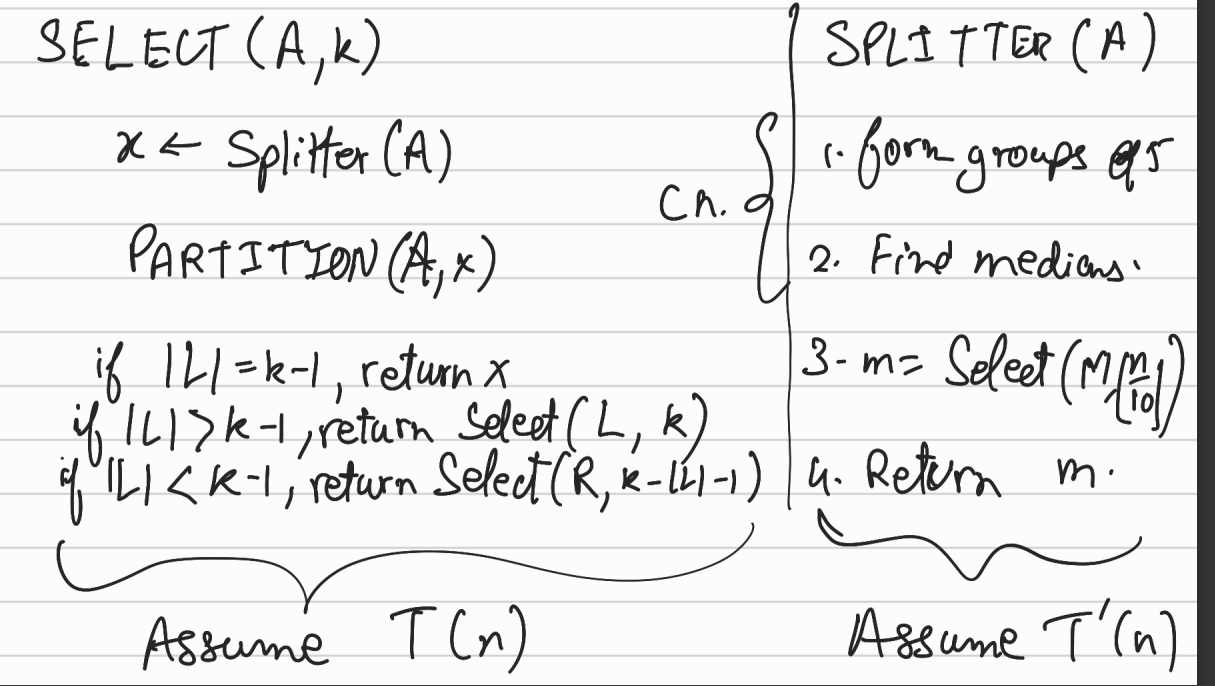
\includegraphics[width=0.5\textwidth]{alg2.PNG}
  \caption{Pseudocode for Analysis of median of median selection algorithm}
  \label{fig:algorithm}
\end{figure}
From Figure \ref{fig:algorithm}, assume the running time of the SELECTION algorithm to be $T(n)$ and that of the SPLITTER to be $T'(n)$. Then,
\begin{equation*}
    T(n) \leq T'(n) + T\left(\frac{5n}{7}\right)
\end{equation*}
And,
\begin{equation*}
    T'(n) \leq T\left(\frac{n}{7}\right) + cn
\end{equation*}

Combining both the equations together we get,
\begin{equation*}
    T(n) \leq T(5n/7) + T(n/7) + cn
\end{equation*}

since ((5n/7)+(n/7)) is less than n, it is contracting and can be solved. 

Now proof by induction, assuming $T(n) \leq 7cn$\\

Base Case:\\
\begin{equation*}
    T(1) \leq 7c
\end{equation*}
This is true as we can select 1 element from an array of size 1 in constant time.\\

Next, we assume it is true for any k < n. So, it is true for T(n/7) and T(5n/7)\\

Finally, for T(n)
\begin{eqnarray*}
    T(n) &\leq& T(5n/7) + T(n/7) + cn\\
    &\leq& 5cn + cn + cn \\
    &\leq& 7cn
\end{eqnarray*}
This concludes $T(n) \in O(n)$


\section*{Exercise 3}
\subsection*{(a)}

If we have only 1 phone, then we must go through each floor incrementally because otherwise if we skip a floor and our phone breaks, we will not know for sure whether the threshold value was the floor where the phone broke or the floor before it. So, we will need something like the following process:
\begin{verbatim}
1. function find_threshold(n):
2.     for i from 0 to n:
3.         if does_phone_break(i):
4.             return (i - 1)
\end{verbatim}
It is trivial to see that there is one for loop which loops for n times in worst case, that in the worst case, $T(n) \in \Theta (n)$

\subsection*{(b)}
To solve this, let us imagine splitting our floors into $\sqrt{n}$ segments of size $\sqrt{n}$ each ($\sqrt{n}\times \sqrt{n} = n$). We drop the first phone from the highest floor of each segment going from the segment at the bottom of the building. When the phone breaks, it will inform us which segment has the threshold floor k. We can then use the second phone to go through each floor in that segment in orderly fashion. This process is shown below in code.
\begin{verbatim}
1. function find_threshold(n):
2.     steps = floor(sqrt(n))
3.     current_floor = 0
4.     while current_floor < n:
5.         if phone_breaks(floor_no = current_floor):
6.             break
7.         current_floor += steps
8.     for i from (current_floor - steps) to (current_floor - 1):
9.         if phone_breaks(floor_no = i)
10.            return i
\end{verbatim}

In line 2, square root can be calculated in O(log log n). \\
Line 3 runs in constant time. \\
The loop from line 4 to 7 will run for $\sqrt{n}+1$ at worst.
The loop from line 8 to 10 will run for $\sqrt{n}$ times.
In summary, 

\begin{eqnarray*}
    T(n) & \leq & \log{\log{n}} + c + (\sqrt{n}+1) + \sqrt{n}\\
    & \leq & \log{\log{n}} + c + 2 \cdot \sqrt{n} + 1\\
\end{eqnarray*}

Therefore, $T(n) \in \Theta(n^{(1/2)})$

\subsection*{(c)}
The core idea is very similar to the solution to part (b) and the same as a binary search. We divide the n floors into $n^{1/t}$ segments each of length $n^{(t-1)/t}$ size. Then, we further divide these segments into $n^{1/t}$ segments. We keep repeating this process (t-1) times until the smallest segments are of the size $n^{1/t}$. In this case, we once again, start at the outer most layer and start dropping our phone to determine the next segment. Consider the algorithm below:

\begin{verbatim}
1.    function find_threshold(n, t, start = 1):
2.        steps = floor(length(start-n)^(1/t))
3.        current_floor = start
4.        if steps <= 1:
5.            for i from (current_floor) to (n):
6.                if phone_breaks(floor_no = i)
7.                    return i
8.        while current_floor < n:       
9.            if phone_breaks(floor_no = current_floor):
10.               find_threshold(current_floor, t, start = current_floor - steps)
11.           current_floor += steps
\end{verbatim}

Line 2 can be computed in constant time using Newton's method depending on the precision required. Line 3 takes constant running time. Lines 4 to 7 compute the base case and take $O(n^{1/t})$ time to run. Lines 8 to 11 loop over endpoints of the segment and in the worst case, it runs for $n^{1/t}$ times before it recurses over a problem of size $n^{(t-1)/t}$. So, our recurrence relation is:\\
\begin{equation*}
    T(n) = T(n^{(t-1)/t}) + O(n^{1/t}) + c
\end{equation*}
We could solve this recursion, but it is trivial to see that in the worst case scenario, we must loop through the sets of size $n^{1/t}$ for $t$ times as there will be $t$ layers in total and hence $t$ recursion calls in total. Hence, the total time complexity will be $O(tn^{1/t})$. This is not a very tight bound as the value of $n$ decreases at every loop. \\
For the specific case when $t = \lceil\log_2(n)\rceil$, our algorithm reduces to the more familiar case of binary search. But if we have even more phones than that i.e., $t \geq \lceil\log_2(n)\rceil$, we wouldn't even need all the phones to check for the threshold. 

\subsection*{(d)}
In the analysis of part (b), we have been a bit loose. Imagine, instead of dividing the floors into segments of size $\sqrt{n}$, we divide them into segments of size $\sqrt{k}$. We still do the same thing, start by dropping the phone from the bottom floor in increments of $\sqrt{k}$. When that phone breaks, we then start from the last checked floor one by one until we find the threshold. The reason this works is that the first floor will only need to be dropped $\sqrt{k}$ times at max, because $\sqrt{k}\times \sqrt{k} = k$. So, if we drop the first phone more than $\sqrt{k}$ times, we don't gain any more information. Hence, total phone drops required are $\sqrt{k}$ drops for first phone and $\sqrt{k}$ drops for 2nd floor. This gives us the time complexity of $O(\sqrt{k})$. Of course, the caveat here is that it is almost impossible to guess the exact value of k. But if we knew k, then we could confirm the threshold again in $O(\sqrt{k})$ time.


\end{document}